

\chapter{التصميم البرمجي والتنجيز}
نبيّن في هذا الفصل التصميم البرمجي للنظام وطريقة تنجيزه والأدوات المستخدمة لذلك.
ونقوم بشرح مخططات الصفوف للحزم البرمجية.
وسرد القرارات التصميمة المعتبرة والأنماط التصميمية \eng{Design Patterns} المستخدمة.
ننوه إلى أن الرماز البرمجي وجميع الحزم البرمجية موجودة تحت المجلد \eng{src}.
todo




\section{قراءة المعطيات}
تم بناء الحزمة \eng{datasets} للتعامل مع المعطيات. أي لقراءة النصوص وكتابة الميزات.
تحوي هذه الحزمة صف وحيد \eng{Document} وهو الصف الأساسي المستخدم ليحمل معلومات النص مثل اسمه ومساره وغيرها.
يبيّن الشكل~\ref{fig:cd:datasets} مخطط الصفوف لهذه الحزمة.
كما تحوي هذه الحزمة حزمتين جزئيتين هما الحزمة \eng{corpora} والحزمة \eng{writers}.

\begin{figure}[htb]
	\centering
	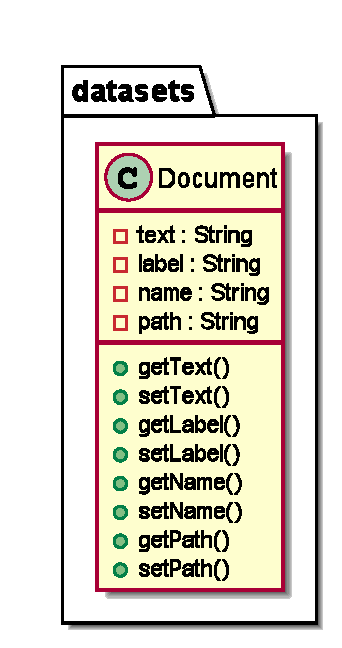
\includegraphics[width=0.25\linewidth]{images/cd-datasets.eps}
	\caption{%
		مخطط الصفوف للحزمة \eng{datasets}.
	}
	\label{fig:cd:datasets}
\end{figure}

الحزمة \eng{corpora} فيها مجموعة من الصفوف المستخدمة لقراءة مجموعة كبيرة من النصوص والمرور عليها ومعالجتها.
إذ أن الصفوف خارج هذه الحزمة تستخدم الواجهة \eng{TextCorpus}.
ويمكن توسيع هذه الحزمة بإنشاء صف جديد ينجّز هذه الواجهة.
حيث يجب أن يعرّف آلية الحصول على النصوص المكتوبة وتصنيفاتها.
تم استخدام النمط التصميم \eng{Iterator design pattern} لتحقيق ذلك.
إذ وجدناه مناسباً ويقوم بتأدية الغرض اللازم.
يبيّن الشكل~\ref{fig:cd:corpora} مخطط الصفوف لهذه الخزمة.

\begin{figure}[htb]
	\centering
	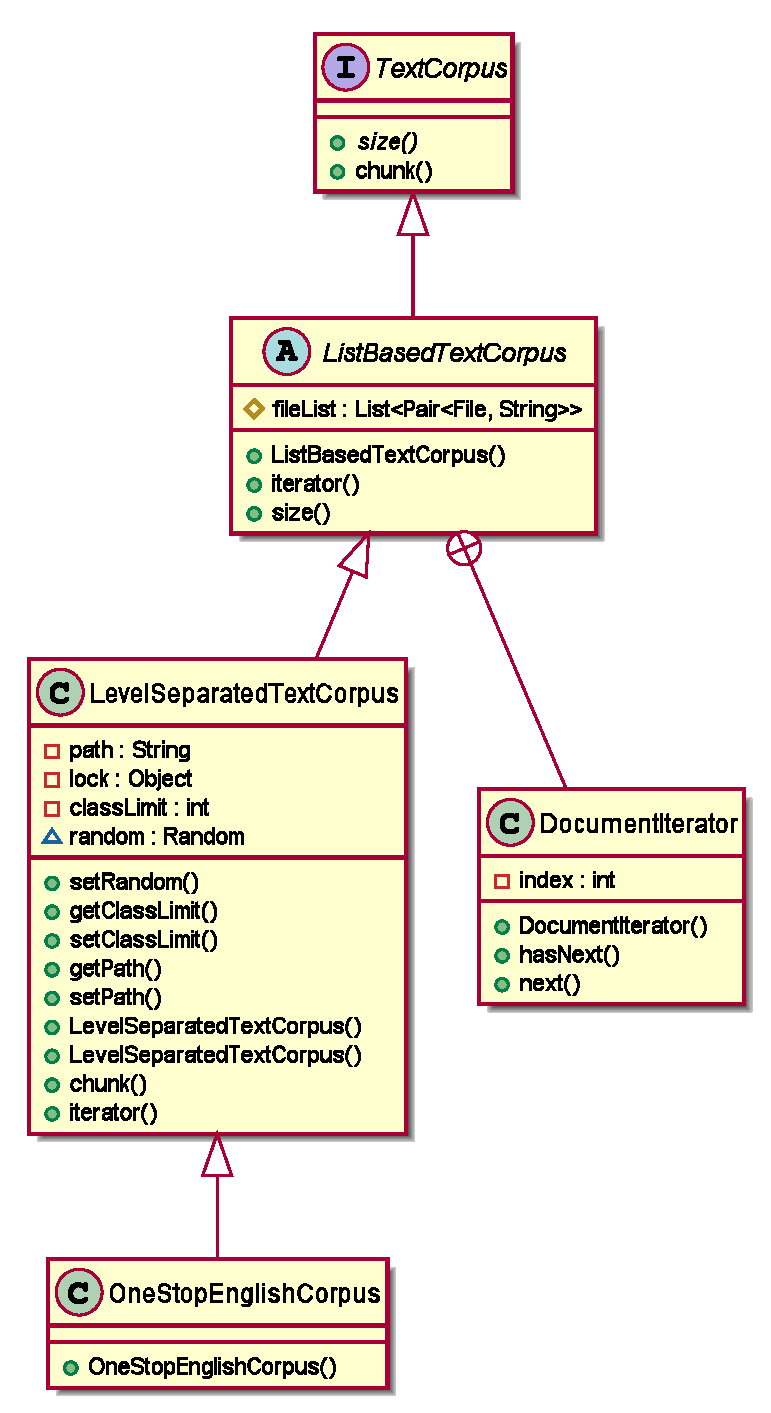
\includegraphics[width=0.6\linewidth]{images/cd-corpora.eps}
	\caption{%
		مخطط الصفوف للحزمة \eng{datasets.corpora}.
	}
	\label{fig:cd:corpora}
\end{figure}

وتم بناء الحزمة \eng{writers} لكتابة ملف فيه الميزات التي تم استخراجها من هذه النصوص.
يبيّن الشكل~\ref{fig:cd:writers} مخطط الصفوف لهذه الحزمة.
الواجهة الأساسية الذي يتم استخدامها خارج هذه الحزمة هي \eng{FeatureWriter}.
الصف المكتوب والذي ينجزها يقوم بكتابة الميزات على ملف بلاحقة \eng{CSV (Comma Separated Values)}.
يمكن بإضافة صف ينجز هذه الواجهة تعريف آلية لكتابة الميزات بأي لاحقة أخرى بحسب المطلوب كـ \eng{XML} مثلاً.

\begin{figure}[htb]
	\centering
	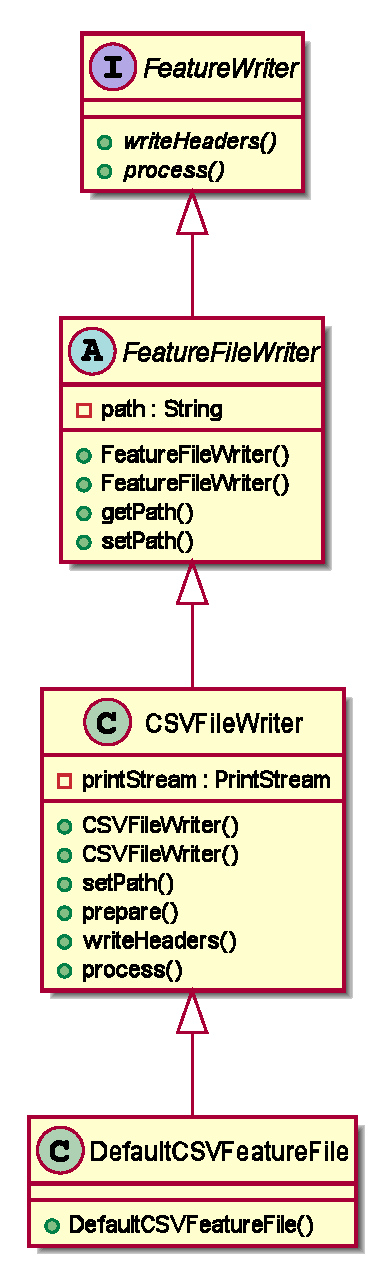
\includegraphics[width=0.25\linewidth]{images/cd-writers.eps}
	\caption{%
		مخطط الصفوف للحزمة \eng{datasets.writers}.
	}
	\label{fig:cd:writers}
\end{figure}





\section{استخراج الميزات}









